\section{Machine Learning Module}
\label{sec:ml}
\emph{In short: classifiers trained on weak labels from the mass spectrum (there are no true labels) reach a test AUC of $0.86$; a cut on their score leaves $\Araw$ unchanged, and an adaptive partition of the Dalitz plane shows the same pattern as the fixed binning.}
As a complementary, data-driven approach to the signal/background separation of the mass fits (Secs.~\ref{sec:frequentist}--\ref{sec:bayesian}), supervised classifiers were trained on weak labels derived from the mass spectrum, and used to study whether an ML-assisted event selection changes $\Araw$ or the mass spectrum, and whether an adaptive partition of the Dalitz plane resolves local structure.

\subsection{Weak Labels and Feature Set}
\label{sec:ml_labels}
\emph{In short: a classifier separates a signal-enriched window from the mass sidebands ($15{,}130$ signal-like and $1940$ background-like candidates, $20$ features, $60/20/20$ split); by the Neyman-Pearson argument of the CWoLa approach it is also the signal/background classifier, if the features carry no information on the mass.}
No candidate carries a true signal/background label, so the classifiers are trained with weak labels, following the classification-without-labels (CWoLa) approach~\cite{cwola}: a classifier is trained to separate two \emph{mixed} samples with different signal fractions, here a signal-enriched window around the $B$ peak and the mass sidebands. If, within each class, the feature distributions are the same in the two samples, the optimal classifier between the two mixtures is a monotonic function of the signal-to-background likelihood ratio $p_s(x)/p_b(x)$, which by the Neyman-Pearson lemma is the most powerful test statistic for signal against background: the classifier trained on the mixtures is also the optimal signal/background classifier~\cite{cwola}. Two conditions follow. The background in the sidebands must be representative of the background under the peak; and the features must not be correlated with the $B$ mass. The second condition cannot hold exactly: the reconstructed mass is not an input feature, but the nine momentum components of the three kaons determine it, so a flexible model can partly learn the mass, separate the two mass regions rather than signal from background, and \emph{sculpt} the mass distribution of the candidates that pass a cut on its score. Section~\ref{sec:ml_stability} tests this directly.

The labels use the nominal Bayesian fit (Sec.~\ref{sec:bayes_posterior}, $\mu=5284.39$, $\sigma=18.00\,\MeV$). Candidates with $|m-\mu|<2\sigma$, $m\in[5248.4,5320.4]\,\MeV$, are labeled signal-like ($15{,}130$); candidates in $[5150,\mu-4\sigma]\cup[\mu+4\sigma,5600]=[5150,5212.4]\cup[5356.4,5600]\,\MeV$ are labeled background-like ($1940$); the $2$--$4\sigma$ gap is left unlabeled. The region $5100$--$5150\,\MeV$, inside the fit window, is excluded from the background-like class to satisfy the first condition: there the background rises towards partially reconstructed $B$ decays (Sec.~\ref{sec:data_mass}), whose kinematics differ from those of the combinatorial background under the peak. The classes are imbalanced ($1940/15{,}130=0.128$). Every model is trained with the same balanced class weights, $w_c=N/(2N_c)$, i.e.\ $4.40$ for background-like and $0.56$ for signal-like candidates (through \texttt{class\_weight} for the scikit-learn models and the network, and through sample weights for gradient boosting), so that the two classes contribute equally to the loss. (Down-sampling the signal-like class and up-weighting it afterwards would have the same effect with less training data; the weights keep all candidates.)

The feature set consists of the 6 per-track kinematic/PID variables (\texttt{PX}, \texttt{PY}, \texttt{PZ}, \texttt{ProbK}, \texttt{ProbPi}, \texttt{IPChi2}) for each of the 3 final-state tracks (18 features), plus two $B$-candidate variables not used in the preselection: \texttt{B\_FlightDistance} and \texttt{B\_VertexChi2}, standard discriminants against combinatorial background (a genuine $B$ flies further before decaying and has a better-reconstructed vertex than a random track combination). Both separate the weak-label classes (Kolmogorov-Smirnov $p<10^{-60}$) and are not redundant with the per-track features (Spearman $|\rho|\leq0.53$ with each of the 18), giving $20$ features. A principal-component analysis of the standardized features needs $15$ of $20$ components to reach $90\%$ of the variance, so no dimensionality reduction is applied; with $20$ features and $\sim10^4$ training candidates the sample is not in the regime where the distance-based methods suffer from the curse of dimensionality. The labeled sample was split $60/20/20$ into training, validation and test sets ($10{,}242/3414/3414$ candidates, $388$ background-like in the test set), stratified on the label, with the feature scaler fit on the training set only.

\subsection{Model Comparison}
\label{sec:ml_models}
\emph{In short: six classifiers; the tree ensembles and the neural network reach test AUC $0.857$--$0.864$, about $0.09$ above the linear models and indistinguishable from each other within the test-set uncertainty ($0.012$); gradient boosting, best in cross-validation, is the reference.}
\begin{table}[h]
\centering
\begin{tabular}{lccc}
\toprule
Model & CV AUC & Test AUC & Brier \\
\midrule
Logistic Regression       & $0.769 \pm 0.016$ & $0.771 \pm 0.013$ & $0.197$ \\
Logistic Regression (L1)  & --                & $0.771 \pm 0.013$ & $0.198$ \\
Decision Tree             & $0.816 \pm 0.011$ & $0.824 \pm 0.013$ & $0.133$ \\
Random Forest             & $0.863 \pm 0.017$ & $0.860 \pm 0.012$ & $0.122$ \\
Gradient Boosting         & $\mathbf{0.866 \pm 0.016}$ & $0.864 \pm 0.012$ & $0.116$ \\
FFNN                      & --                & $0.857 \pm 0.012$ & $0.134$ \\
\bottomrule
\end{tabular}
\caption{Cross-validated AUC (mean and standard deviation over the folds), test-set AUC (with bootstrap uncertainty) and test-set Brier score of the raw scores. Gradient boosting, best in cross-validation, is the reference model. The FFNN is validated on the validation set instead of by cross-validation.}
\label{tab:ml_models}
\end{table}

Six classifiers were trained: logistic regression, without and with an $L1$ penalty (linear baselines), a decision tree (depth 4, fixed in advance as a shallow, interpretable baseline and not pruned), a Random Forest~\cite{breiman_rf} (300 trees of depth 8), gradient boosting~\cite{friedman_gbm} (200 stages of depth-3 trees, learning rate $0.05$), and a feed-forward neural network (FFNN: two hidden layers of 32 and 16 units with ReLU activation, dropout $0.2$, binary cross-entropy, the Adam optimizer~\cite{adam} with learning rate $10^{-3}$, early stopping on the validation AUC, sigmoid output). The linear models and the network are parametric, with a fixed number of parameters, and the trees and ensembles non-parametric, whose complexity grows with the data; the more flexible models are less interpretable, which is why the linear and single-tree baselines are kept. Both the logistic-regression log-loss and the network's binary cross-entropy are the negative log-likelihood of a Bernoulli distribution with probability $p(x)$, the same quantity minimized by the mass fits. The models are compared through the area under the receiver operating characteristic (ROC) curve (AUC), which equals the probability that a randomly chosen signal-like candidate receives a higher score than a randomly chosen background-like one ($0.5$ for a random classifier, $1$ for a perfect one). Table~\ref{tab:ml_models} gives the 5-fold cross-validated AUC on the training set and the AUC on the untouched test set, with its bootstrap uncertainty. The reference model for the rest of the section was chosen on the cross-validated AUC, so that the test set is not used for any choice: gradient boosting ($0.866$), essentially tied with the Random Forest ($0.863$).



\begin{figure}[h]
\centering
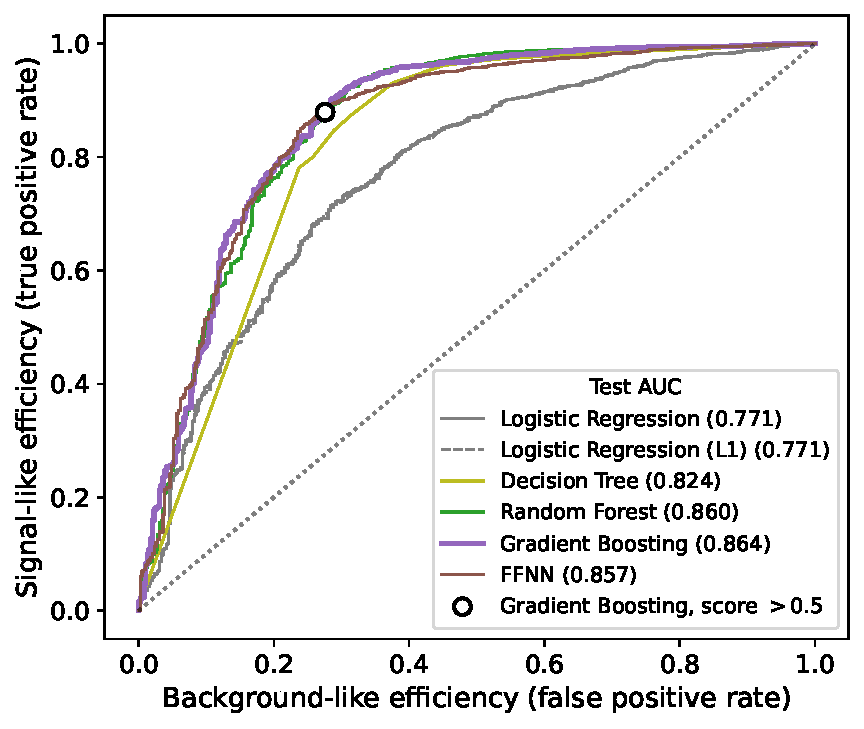
\includegraphics[width=\columnwidth]{figures/ml_nominal_roc.pdf}
\caption{ROC curves on the test set, with the test AUC of each model in the legend (Table~\ref{tab:ml_models}); the reference model is drawn thicker, and the two logistic regressions overlap. The circle marks the cut on the reference score used in Sec.~\ref{sec:ml_stability}.}
\label{fig:ml_roc}
\end{figure}

The three non-linear ensembles and the FFNN improve the AUC by $\sim$0.09 over the linear models and by $\sim$0.04 over the single tree (Fig.~\ref{fig:ml_roc}), while their mutual differences ($\leq0.007$) are smaller than the test-set uncertainty ($0.012$). The FFNN training is reproducible (fixed seeds, deterministic operations); its dependence on the random initialization, measured by retraining it with ten seeds, is $0.854\pm0.005$ in test AUC.



\begin{figure*}[t]
\centering
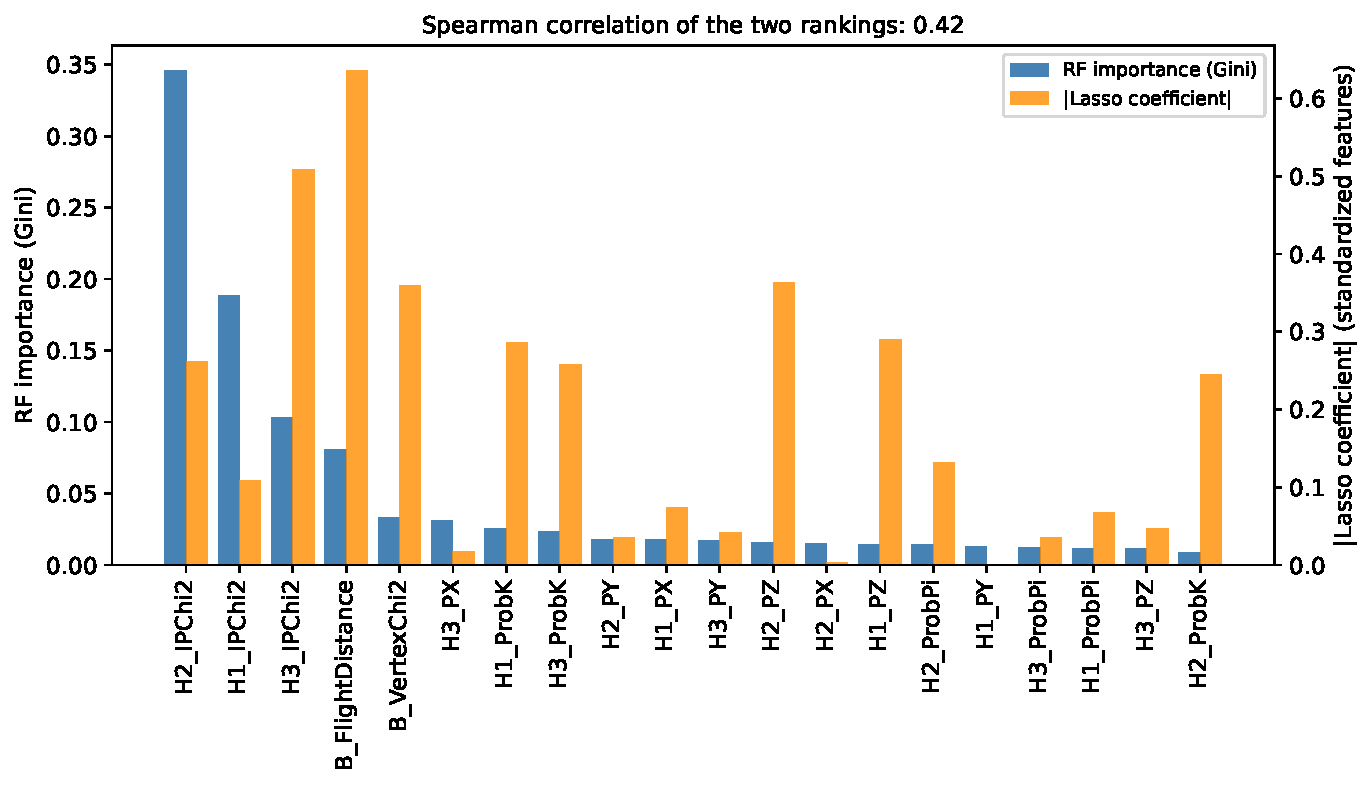
\includegraphics[width=0.95\textwidth]{figures/ml_nominal_features.pdf}
\caption{Random Forest feature importance (Gini, a) and magnitude of the Lasso coefficient of the standardized feature (b) for the 20 features, both ordered by Random Forest importance; the two $B$-candidate variables are highlighted.}
\label{fig:ml_features}
\end{figure*}

The two measures of the relevance of a feature available here -- the Random Forest importance (the decrease in Gini impurity $G=1-\sum_c p_c^2$, $p_c$ the class fractions in a node, produced by the splits on that feature) and the magnitude of the $L1$-regularized (Lasso~\cite{tibshirani_lasso}) logistic-regression coefficient of the standardized feature -- agree only partly (Fig.~\ref{fig:ml_features}; Spearman correlation of the two rankings $0.42$, $p=0.06$). The impact-parameter variables \texttt{IPChi2} dominate the Random Forest, while the Lasso coefficients are largest for \texttt{B\_FlightDistance}, \texttt{H3\_IPChi2}, \texttt{H2\_PZ} and \texttt{B\_VertexChi2}. The difference is expected: the Gini importance reflects the use of a feature in non-linear splits and interactions, and is shared among correlated features, while a linear coefficient measures the effect of a feature with the others held fixed. Both measures rank the two $B$-candidate variables among the top five (Random Forest 4th and 5th, Lasso 1st and 4th): they summarize in one number the displaced-vertex topology that the per-track variables encode only jointly.



\subsection{Regularization, Bias-Variance, and Calibration}
\label{sec:ml_regcal}
\emph{In short: the linear model does not overfit, gradient boosting overfits beyond $\sim$150 stages without losing test AUC, and class weights bias the probabilities, which an isotonic recalibration corrects (Brier score $0.122\to0.062$) without changing the ranking.}
A scan of the regularization strength of the logistic regression (penalties and loss functions are defined in Appendix~\ref{app:theory}) ($30$ log-spaced values of $C=1/\alpha$, cross-validated) gives the same optimal AUC for the $L1$ and $L2$ penalties ($0.7686$, at $C_{L1}=0.12$ and $C_{L2}=9.2$), and the optimal $L1$ penalty sets no coefficient to zero: the linear model does not overfit, and its limitation is the linear decision boundary, not the variance.

\begin{figure*}[t]
\centering
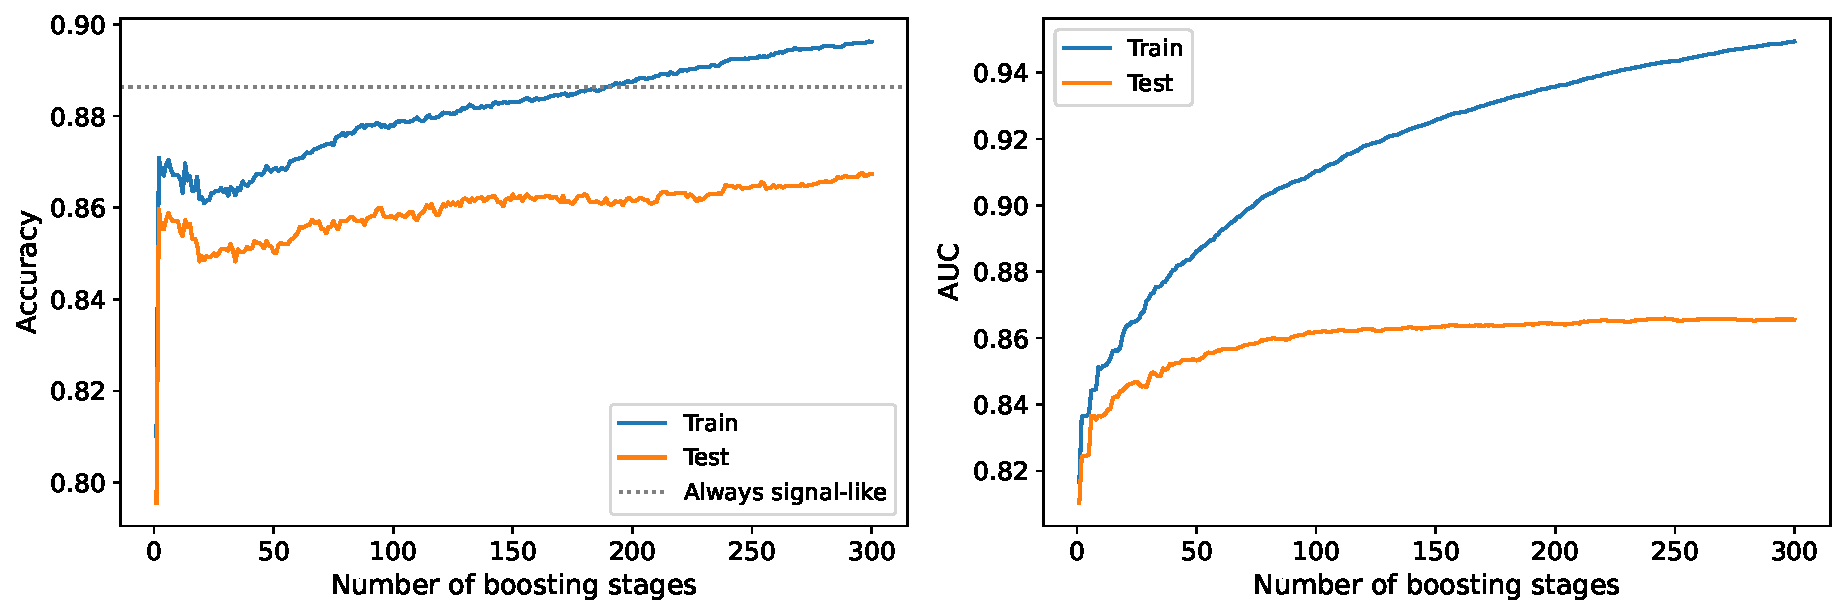
\includegraphics[width=0.95\textwidth]{figures/ml_nominal_bias_variance.pdf}
\caption{Gradient boosting: (a) accuracy at the $0.5$ threshold and (b) AUC on the training and test sets as a function of the number of boosting stages. The dotted line is the accuracy of always predicting the signal-like class.}
\label{fig:ml_bias_variance}
\end{figure*}

\begin{figure}[t]
\centering
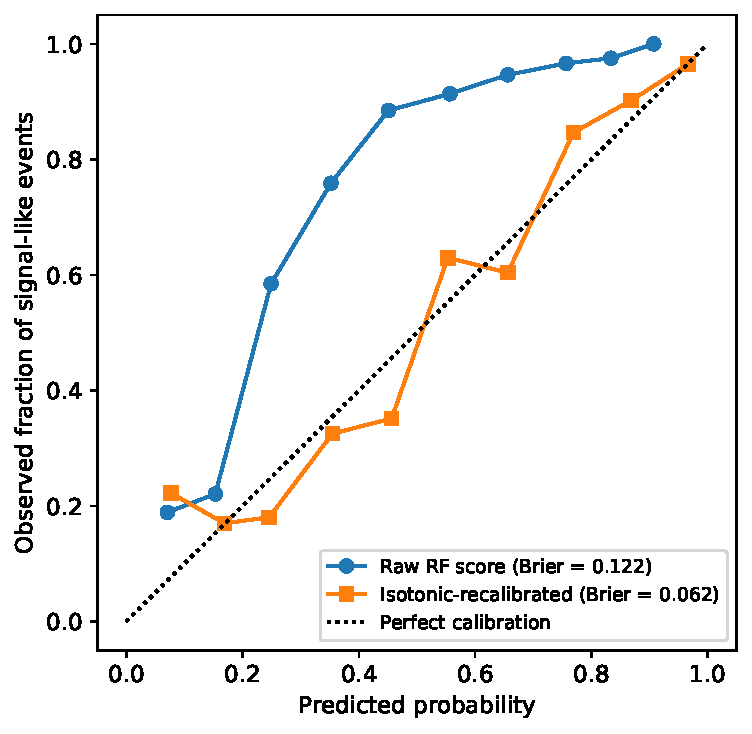
\includegraphics[width=\columnwidth]{figures/ml_nominal_calibration.pdf}
\caption{Reliability diagram of the Random Forest on the test set: observed fraction of signal-like candidates vs.\ predicted probability, for the raw score (with binomial uncertainties) and for the isotonic-recalibrated one. Bottom: distribution of the raw score for the two weak-label classes; the low-probability bins contain few candidates.}
\label{fig:ml_calibration}
\end{figure}

The bias-variance trade-off was studied with gradient boosting, whose complexity grows with the number of boosting stages (Fig.~\ref{fig:ml_bias_variance}). The test AUC rises up to $\sim$150 stages and then stays at $0.865$, while the training AUC keeps rising: the train-test gap grows from $0.018$ at 20 stages to $0.084$ at 300. The additional stages fit fluctuations of the training sample without improving the ranking of new candidates -- overfitting, which the default 200 stages of Table~\ref{tab:ml_models} do not reach in the test AUC. The test accuracy at the $0.5$ threshold stays below that of always predicting the majority class ($0.886$): with balanced class weights the classifier is trained to minimize the weighted error, in which a misclassified background-like candidate counts eight times more than a signal-like one, and not the unweighted error rate.




The AUC depends only on the ranking of the scores; whether a score can be read as a probability is measured by the Brier score~\cite{brier}, $\mathrm{BS}=\frac{1}{N}\sum_i (p_i-y_i)^2$, the mean squared difference between predicted probability $p_i$ and label $y_i\in\{0,1\}$ (lower is better). Class weights change the probabilities a model learns: a classifier trained with weights $w_s,w_b$ on the two classes converges to
\[
\tilde p=\frac{w_s p}{w_s p+w_b(1-p)}
\]
instead of the true $p$, i.e.\ it describes a world in which the classes are re-balanced. With $w_b>w_s$ the raw scores therefore \emph{underestimate} the probability of the signal-like class, which is what the reliability diagram of the Random Forest shows (Fig.~\ref{fig:ml_calibration}): at a raw score of $0.25$ the observed signal-like fraction is already $0.58$. An isotonic recalibration~\cite{zadrozny_elkan}, fitted on held-out folds of the unweighted training sample, follows the diagonal and halves the Brier score, from $0.122$ to $0.062$ (the Brier score is the mean squared error of the predicted probability against the $0/1$ label). Most of the gain undoes the re-weighting rather than correcting the model; the ranking, and hence the AUC and any selection based on a score threshold, is unchanged by a monotonic recalibration.



\subsection{Uncertainty Quantification}
\label{sec:ml_uncertainty}
\emph{In short: the three estimators give mean per-candidate uncertainties of $0.178$ (Random Forest), $0.095$ (MC dropout) and $0.050$ (deep ensemble); they measure different sources of variability, and only the Random Forest spread visibly decreases with the training-set size.}
\begin{figure*}[t]
\centering
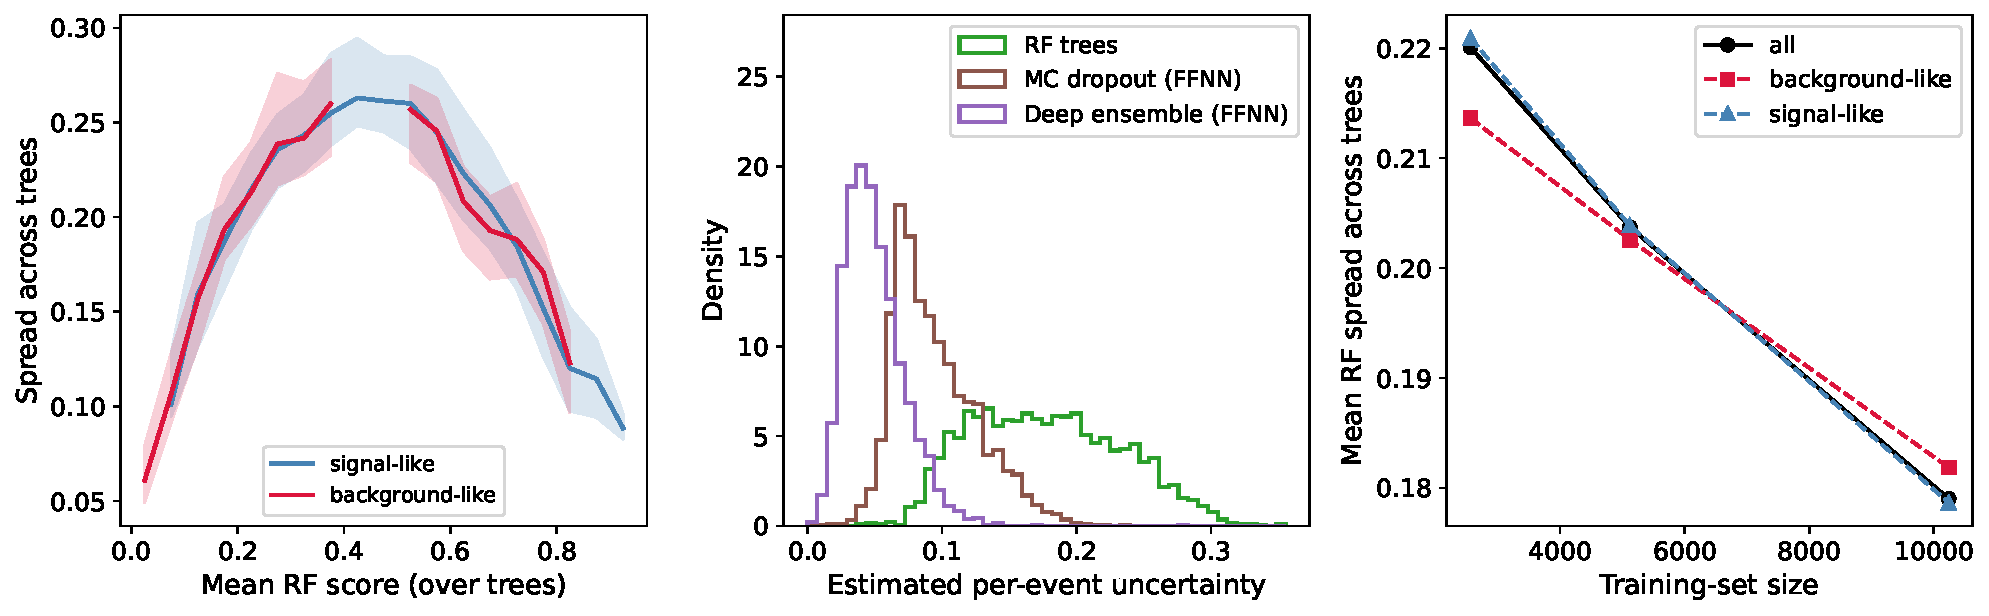
\includegraphics[width=0.95\textwidth]{figures/ml_nominal_uncertainty.pdf}
\caption{(a) Spread across the Random Forest trees vs.\ mean tree score, median and 16--84\% band of the test candidates of each weak-label class. (b) Distributions of the per-candidate uncertainty from the Random Forest trees, MC dropout and the deep ensemble. (c) Mean Random Forest spread vs.\ training-set size, for all, background-like and signal-like test candidates.}
\label{fig:ml_uncertainty}
\end{figure*}

The uncertainty of a prediction has two components: \emph{aleatoric}, from the intrinsic overlap of the classes in feature space, which more training data cannot reduce, and \emph{epistemic}, from the limited knowledge of the model parameters, which more training data reduces. Three estimators were compared, each giving an ensemble of $M$ predictions $p_m(x)$ for each candidate and quoting their spread, $\sigma(x)=\big[\frac1M\sum_m (p_m(x)-\bar p(x))^2\big]^{1/2}$: the $M=300$ trees of the Random Forest, each trained on a bootstrap sample; $M=300$ forward passes of the FFNN with dropout kept active at inference (MC dropout), which approximates sampling from a Bayesian posterior over the network weights~\cite{gal_mcdropout} (a full Bayesian network trained by variational inference was not used: it needs a dedicated implementation and MC dropout gives the same kind of ensemble at no extra cost); and a deep ensemble~\cite{deep_ensembles} of $M=10$ FFNNs trained from different random initializations. The mean per-candidate uncertainty is $0.178$ for the Random Forest, $0.095$ for MC dropout ($0.099\pm0.006$ over the ten initializations) and $0.050$ for the deep ensemble (Fig.~\ref{fig:ml_uncertainty}), with the same values within $10\%$ for background-like and signal-like candidates.

The three estimators answer different questions, which explains the factor $\sim$3.5 between them. The deep ensemble only varies the initialization, on the same training data; MC dropout also perturbs the network structure; the trees of the Random Forest differ in their training data (bootstrap) and in the features they use, and each tree, of limited depth, is individually a poor and discrete estimator of $p$. Their per-candidate values are correlated but not interchangeable (Spearman correlations $0.41$--$0.57$ between pairs). The Random Forest spread contains both components. It is largest for scores around $0.5$ (Fig.~\ref{fig:ml_uncertainty}a), where the classes overlap and the trees disagree most -- an aleatoric contribution; and it decreases with the size of the training set, from $0.220$ with a quarter of it to $0.204$ with half and $0.179$ with the full set, while the test AUC stays at $0.860$--$0.862$ -- the epistemic contribution, which more data reduces.



\subsection{K-means on the Dalitz Plot}
\label{sec:ml_kmeans}
\emph{In short: for $K=8$ two clusters deviate by more than $3\sigma$ ($\chi^2=46.4$ for $7$ degrees of freedom): a negative asymmetry at low $m^2_{\mathrm{lo}}$ and positive ones at high $m^2_{\mathrm{hi}}$, as in the fixed binning.}
$K$-means is the unsupervised part of the module: it uses no labels, and the partition of the Dalitz plane is learned from the density of the candidates rather than fixed by hand. As an adaptive alternative to the fixed Dalitz-plot binning of Sec.~\ref{sec:bayes_dalitz}, the candidates of the fit window were partitioned with $K$-means~\cite{lloyd_kmeans} on the two standardized Dalitz variables $(m^2_{\mathrm{lo}},m^2_{\mathrm{hi}})$. $K$-means partitions the points $x_i$ into $K$ clusters $C_k$ minimizing the within-cluster sum of squares (inertia) $W=\sum_k\sum_{i\in C_k}\lVert x_i-\bar x_k\rVert^2$, with $\bar x_k$ the cluster centroids; $K$ has to be fixed in advance. The quality of a partition is measured by the silhouette~\cite{silhouette}: for each point, $s_i=(b_i-a_i)/\max(a_i,b_i)$ compares its mean distance $a_i$ to the other points of its cluster with the mean distance $b_i$ to the points of the nearest other cluster, and the average over all points ($-1\le s\le 1$, higher is better) measures how well separated the clusters are. $K=8$ was fixed in advance, as a compromise between resolution and the number of candidates per cluster (at least $1233$), and $K=3$, the silhouette optimum over $K=2$--$12$ ($0.46$, against $0.41$ for $K=8$, a local maximum), was added. Both partitions are stable: repeating the clustering with a different random initialization gives an adjusted Rand index~\cite{hubert_ari} above $0.998$.

\begin{figure}[h]
\centering
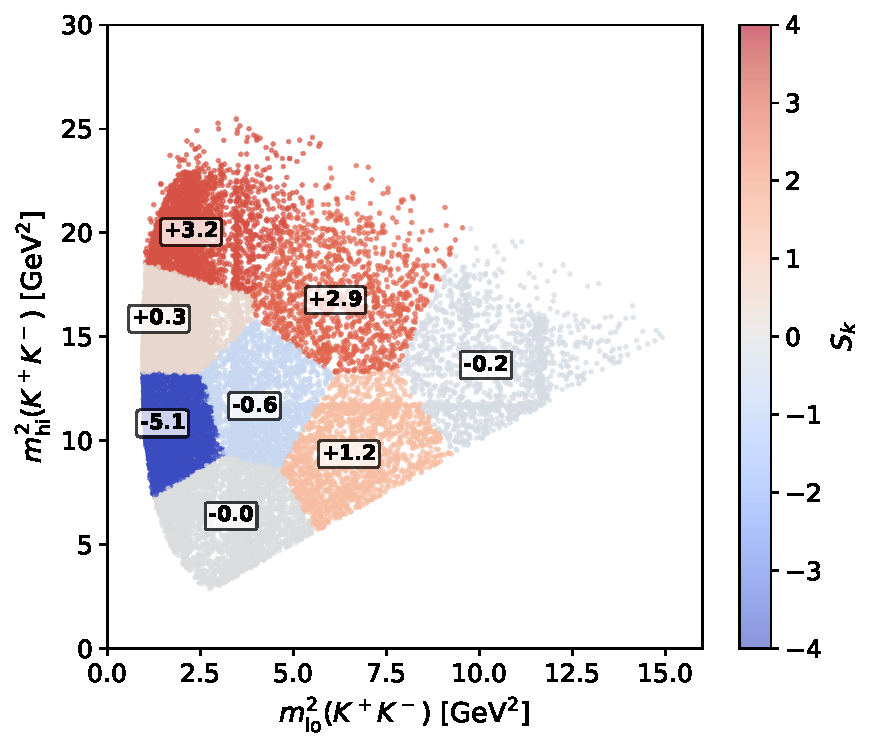
\includegraphics[width=\columnwidth]{figures/ml_nominal_kmeans.pdf}
\caption{$K$-means partition ($K=8$) of the Dalitz plane, all candidates of the fit window, same axes as Fig.~\ref{fig:bayes_dalitz}. Color and labels: local significance of each cluster with respect to the global asymmetry, $S_k=(A_k-A_{\mathrm{glob}})/\sigma(A_k)$, on the same scale as panel (c) of Fig.~\ref{fig:bayes_dalitz}.}
\label{fig:ml_kmeans}
\end{figure}

The asymmetry of each cluster was compared with the global one as in Sec.~\ref{sec:bayes_dalitz}, $S_k=(A_k-A_{\mathrm{glob}})/\sigma(A_k)$. For $K=8$ (Fig.~\ref{fig:ml_kmeans}), two clusters deviate by more than $3\sigma$ (probability $2\times10^{-4}$ for two or more if the asymmetry were uniform), and the homogeneity test gives $\chi^2=46.4/7$ ($p=7\times10^{-8}$). The most significant one lies at low $m^2_{\mathrm{lo}}$ ($1$--$2.5\,\GeV^2$) and intermediate $m^2_{\mathrm{hi}}$, with $A_k=-0.127\pm0.017$ ($n=3601$, $S_k=-5.1$); two clusters at high $m^2_{\mathrm{hi}}$ have positive asymmetries, $A_k=+0.020\pm0.020$ ($S_k=+3.2$) and $+0.040\pm0.028$ ($+2.9$). In the signal window ($|m-\mu|<2\sigma$) the same pattern is sharper -- three clusters beyond $3\sigma$, with $S_k=-5.6$, $+4.4$ and $+3.0$, and $\chi^2=62.3/7$ -- so it is not produced by the background. The coarser $K=3$ partition gives $\chi^2=15.2/2$ ($p=5\times10^{-4}$). The adaptive partition therefore confirms the picture of the fixed binning, a negative local asymmetry at low $m^2_{\mathrm{lo}}$ and positive ones at high $m^2_{\mathrm{hi}}$, with the same caveats (no background subtraction, no correction for detection asymmetries).



\subsection{Stability of $\Araw$ under ML Selection}
\label{sec:ml_stability}
\emph{In short: a cut on the score at $0.5$ keeps $92\%$ of the signal and $36\%$ of the background and leaves $\Araw$ within its expected statistical spread with both fits and with counting; it does not improve the precision and cannot remove the misidentified background.}
\begin{figure}[h]
\centering
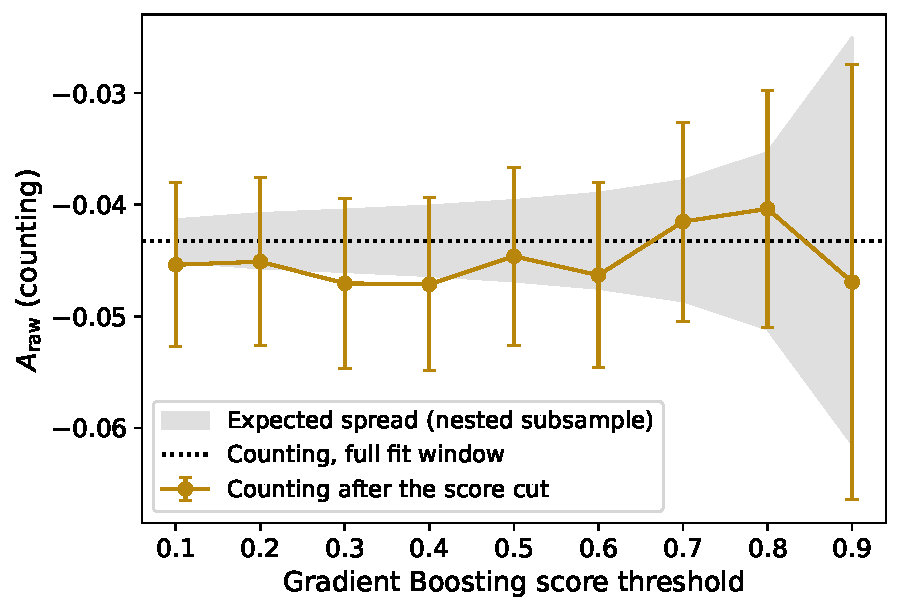
\includegraphics[width=\columnwidth]{figures/ml_nominal_threshold.pdf}
\caption{Counting asymmetry after a cut on the gradient-boosting score, vs.\ threshold, with its binomial uncertainty. Dotted line: counting asymmetry of the full fit window; band: expected statistical spread of a nested subsample around it, $\pm\sqrt{\sigma_{\mathrm{sub}}^2-\sigma_{\mathrm{full}}^2}$.}
\label{fig:ml_threshold}
\end{figure}

The reference (gradient-boosting) score was applied to all candidates of the fit window (on the test set, a cut at $0.5$ keeps $88\%$ of the signal-like and $28\%$ of the background-like candidates, Fig.~\ref{fig:ml_roc}), not only to the labeled ones used in training, and the counting asymmetry was recomputed after cuts on the score from $0.1$ to $0.9$ (Fig.~\ref{fig:ml_threshold}). Since every selected sample is contained in the full one, the expected statistical spread of the difference is $\sqrt{\sigma_{\mathrm{sub}}^2-\sigma_{\mathrm{full}}^2}$, not the uncertainty of either estimate. Over all thresholds, which keep from $18{,}443$ to $2621$ candidates, the shift with respect to the full window ($A_{\mathrm{count}}=-0.0432$) stays within $1.4$ times this spread: the selection does not introduce a detectable bias in the counting asymmetry. Split by magnet polarity at a cut of $0.5$, the counting asymmetries are $-0.060\pm0.010$ (down) and $-0.024\pm0.012$ (up), $2.2\sigma$ apart; the frequentist fit of the same samples, which separates the background, gives $-0.054\pm0.011$ and $-0.032\pm0.013$, $1.3\sigma$ apart (against $0.7\sigma$ for the full sample, Sec.~\ref{sec:bayes_checks}), so most of the larger difference of the counting estimates comes from the background.



\begin{table*}[t]
\centering
\begin{tabular}{lccc}
\toprule
Method & Full sample & Score $>0.5$ & Shift (expected) \\
\midrule
Bayesian fit    & $-0.0443\pm0.0085$ & $-0.0451\pm0.0087$ & $-0.0008\,(0.0018)$ \\
Frequentist fit & $-0.0441\pm0.0085$ & $-0.0447\pm0.0086$ & $-0.0006\,(0.0012)$ \\
Counting        & $-0.0432\pm0.0071$ & $-0.0446\pm0.0080$ & $-0.0014\,(0.0036)$ \\
\bottomrule
\end{tabular}
\caption{$\Araw$ on the full fit window ($19{,}731$ candidates) and after the cut on the gradient-boosting score ($15{,}709$), by the three methods. The expected shift is the statistical spread of a nested subsample, $\sqrt{\sigma_{\mathrm{sub}}^2-\sigma_{\mathrm{full}}^2}$. Counting includes the background.}
\label{tab:three_methods}
\end{table*}

\begin{figure}[h]
\centering
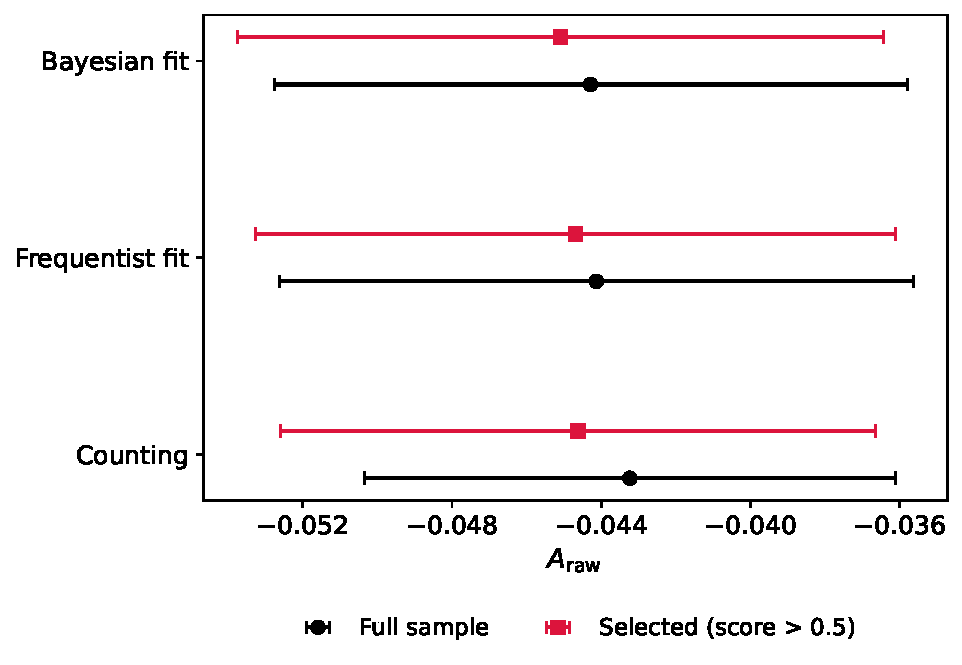
\includegraphics[width=\columnwidth]{figures/ml_nominal_three_methods.pdf}
\caption{$\Araw$ from the Bayesian fit, the frequentist fit and counting, for the full sample and the ML-selected one (Table~\ref{tab:three_methods}).}
\label{fig:ml_three}
\end{figure}

\begin{figure*}[t]
\centering
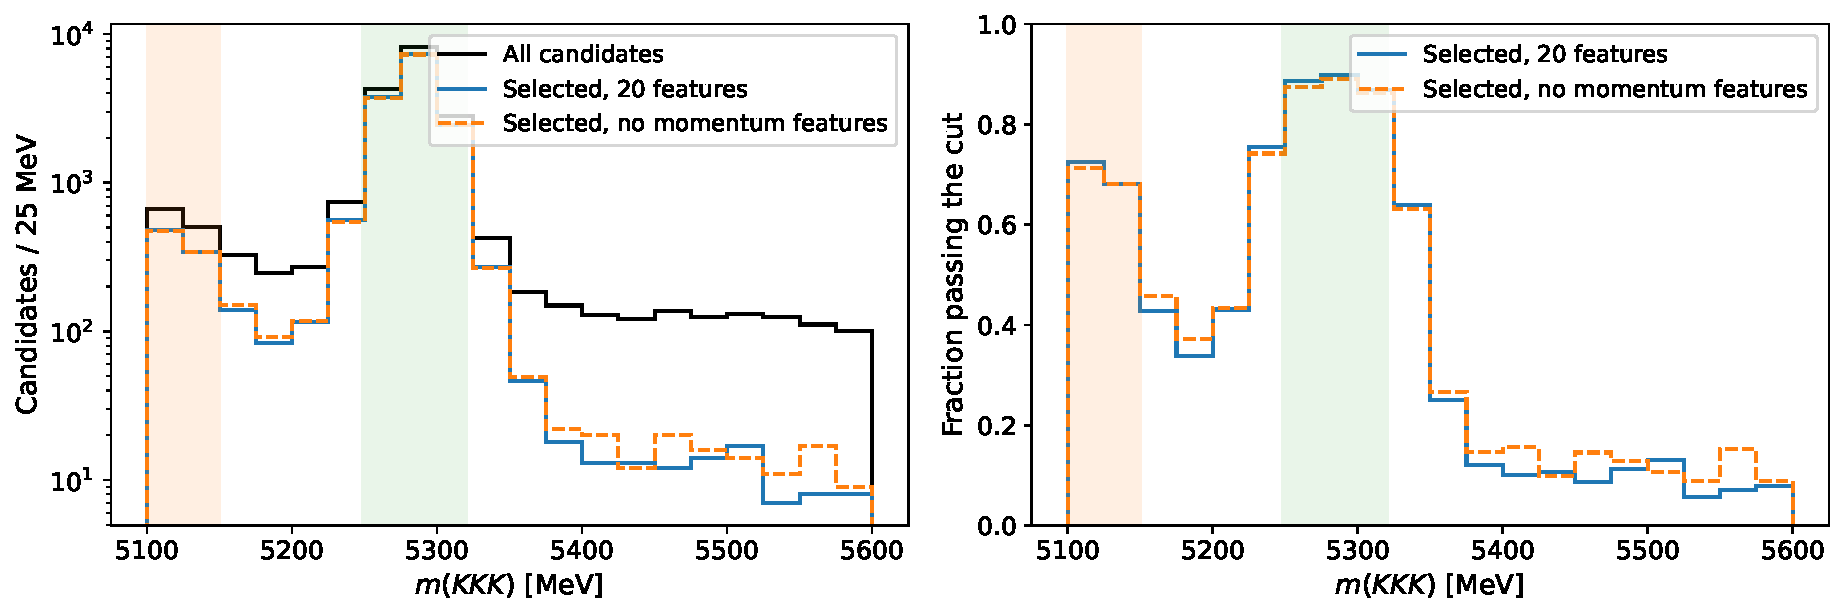
\includegraphics[width=0.95\textwidth]{figures/ml_nominal_mass_after_cut.pdf}
\caption{(a) Mass spectrum of all candidates and of those with gradient-boosting score $>0.5$, for the 20-feature classifier and for one trained without the kaon momentum components (25\,MeV bins). (b) Fraction of candidates passing the cut. Hatched: the region below $5150\,\MeV$ excluded from the background-like labels; grey: the signal-like window.}
\label{fig:ml_mass_cut}
\end{figure*}

Counting cannot reveal whether the selection deforms the mass spectrum. To test this, the selected sample (score $>0.5$, $15{,}709$ candidates) was refitted with the nominal mass model by both inference methods of this work, the Bayesian fit of Sec.~\ref{sec:bayesian} and the frequentist maximum-likelihood fit of Sec.~\ref{sec:frequentist}, and the three estimates were compared with those of the full sample (Table~\ref{tab:three_methods}, Fig.~\ref{fig:ml_three}). The asymmetry is stable: all three shifts are within their expected nested-sample spread, and the significance of $A\neq0$ from the profile likelihood (Wilks' theorem~\cite{wilks}) is $5.2\sigma$ in both samples. The selection keeps $92\%$ of the fitted signal and $36\%$ of the background ($N_s=14{,}121$, $N_b=1590$), but this does not improve the precision on $\Araw$ ($0.0087$ against $0.0085$): the background under the peak is already small ($\approx$4\% in the signal window) and the fit separates it from the signal anyway. The mass spectrum, instead, changes. The goodness of fit of the nominal model degrades from $\chi^2=164/88$ to $253/88$ in the Bayesian fit and from $442/388$ to $557/388$ in the frequentist one (with a different binning), and the background shape changes: the slope of the slow exponential grows from $0.0028$ to $0.0071\,\MeV^{-1}$ ($B^+$) and from $0.0016$ to $0.0057\,\MeV^{-1}$ ($B^-$), and the fraction of the steep one from $0.11$ to $0.28$ and from $0.21$ to $0.50$. Two mechanisms can produce this: the classifier could reconstruct the mass from the kaon momenta and sculpt the background (Sec.~\ref{sec:ml_labels}), or the selection could change the composition of the background. The first is excluded: the same classifier trained without the nine momentum components (test AUC $0.860$) gives the same degradation ($\chi^2=533/388$). The efficiency of the cut as a function of the mass shows the second (Fig.~\ref{fig:ml_mass_cut}): it is $0.89$--$0.90$ at the peak, $\approx0.70$ below $5150\,\MeV$ and $0.06$--$0.13$ above $5375\,\MeV$. The classifier does what it is trained for -- it removes the combinatorial background and keeps genuine $B$ decays, including the partially reconstructed ones and the other non-combinatorial components that the weak labels cannot separate from the signal. In the selected sample these components weigh relatively more, and the nominal model, which has no dedicated component for them, describes it worse, mostly under the peak (the $\chi^2$ of the $\pm4\sigma$ region grows from $75$ to $134$ for 30 bins) and below it. A Crystal Ball signal gives the same degradation ($407\to522$ for 386 degrees of freedom), so it is not due to the signal tails. $\Araw$ is unaffected because it is determined by the peak and the background shape is free in the fit, but a measurement that relied on the background shape, or on a background model taken from the sidebands of the full sample, would be biased by the selection.







\begin{figure*}[t]
\centering
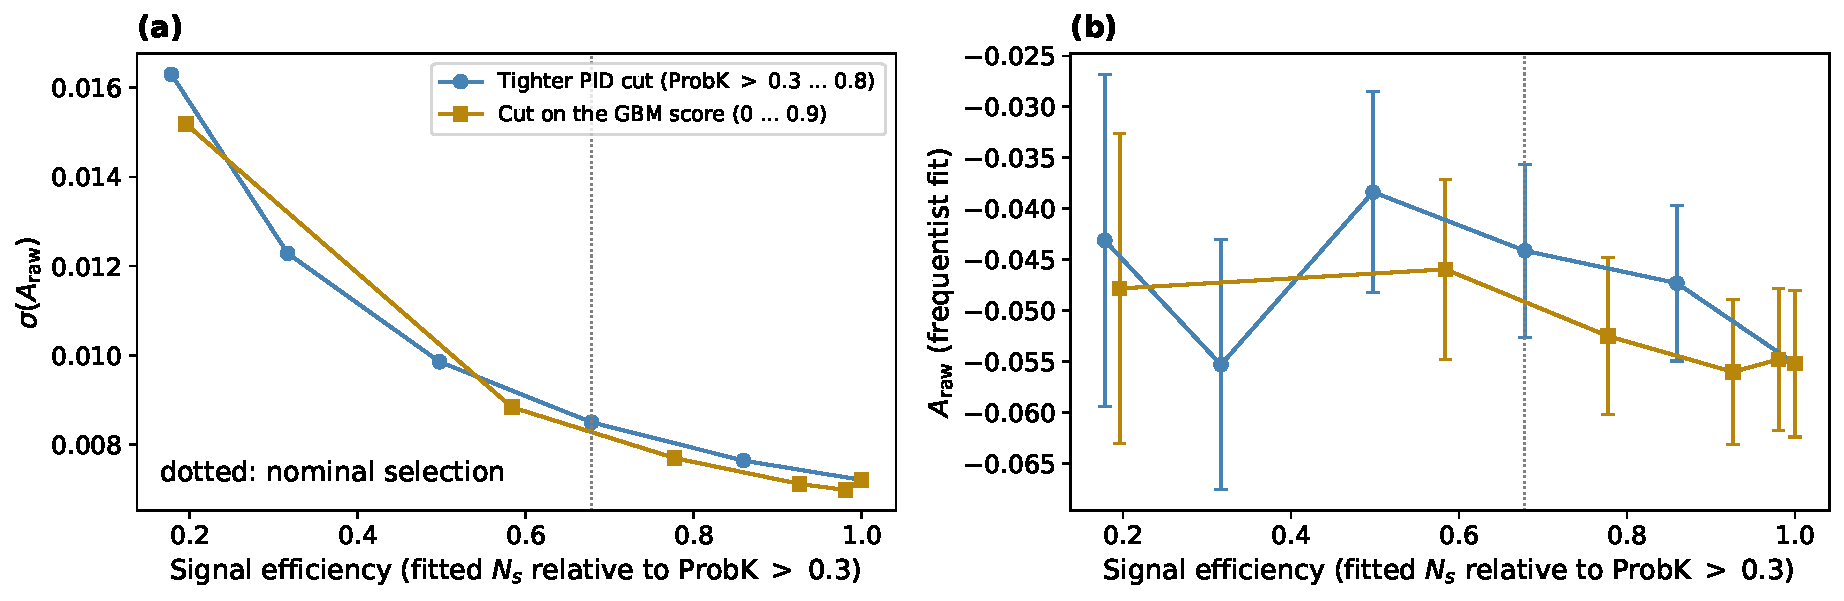
\includegraphics[width=0.95\textwidth]{figures/ml_nominal_high_background.pdf}
\caption{High-background sample ($\texttt{ProbK}>0.3$): (a) statistical uncertainty and (b) value of $\Araw$ from the frequentist fit vs signal efficiency, for tighter identification cuts ($\texttt{ProbK}>0.3,\dots,0.8$) and for cuts on the score of the classifier retrained on this sample ($0,\dots,0.9$). The dotted line marks the nominal selection ($\texttt{ProbK}>0.5$). The samples are nested, so their uncertainties are correlated.}
\label{fig:ml_high_bkg}
\end{figure*}

In the nominal sample the selection cannot improve the precision because there is little background to remove. To test it where the background is larger, the same study was repeated on a sample with a looser kaon identification, $\texttt{ProbK}>0.3$ ($33{,}328$ candidates, signal purity $94\%$ within $\pm2\sigma$ of the peak), with the reference classifier retrained on the weak labels of this sample (test AUC $0.895$). Cleaning it with a cut on the classifier score is compared with tightening the identification cut, at equal signal efficiency (Fig.~\ref{fig:ml_high_bkg}). The classifier removes the combinatorial background with little signal loss -- a cut at $0.5$ keeps $93\%$ of the signal and raises the purity to $99\%$ -- and at any efficiency gives a slightly smaller $\sigma(\Araw)$ than the identification cut. The gain is small ($0.0072\to0.0070$ at best): loosening the identification adds mostly signal ($+47\%$ with respect to the nominal selection), and the background under the peak stays a small fraction. The classifier also cannot remove the background that matters for $\Araw$. With the looser identification the asymmetry moves to $-0.055$, as expected from misidentified $B^\pm\to\pi^\pm K^+K^-$ decays (Sec.~\ref{sec:syst}); tightening the identification cut to $\texttt{ProbK}>0.4$ moves it back by $+0.008$ ($3.3$ times the nested-sample spread), while the score cut that keeps $93\%$ of the signal moves it by $-0.001$. Misidentified $B$ decays peak close to the $B$ mass, so the mass-based weak labels mark them as signal-like: the CWoLa classifier, by construction, cannot learn to reject a background that sits under the peak, and particle identification remains necessary.



\subsection{Hyperparameter Optimization}
\label{sec:ml_hyper}
\emph{In short: the best configurations improve the test AUC by at most $0.005$, less than its uncertainty, and the cross-validated maximum overestimates the test AUC (winner's curse).}
The hyperparameters of the Random Forest ($120$ configurations), gradient boosting ($100$) and the FFNN ($168$: seven architectures, four dropout rates, six learning rates) were optimized by repeated cross-validation on the training set (Tables~\ref{tab:ml_hyperparams}--\ref{tab:ml_ffnn_search}). The best configurations improve the test AUC over the defaults of Table~\ref{tab:ml_models} by $0.005$ (Random Forest), $0.001$ (gradient boosting) and $0.004$ (FFNN), all well below the test-set uncertainty ($0.012$) and, for the FFNN, comparable with its spread over initializations ($0.005$). For the two tree ensembles the best cross-validated AUC is higher than the test AUC of the same configuration ($0.871$ vs $0.866$ and $0.868$ vs $0.865$), as expected when the maximum is taken over many noisy cross-validation estimates (the ``winner's curse''): the selection favors configurations with a favorable fluctuation, and the cross-validated score of the selected configuration is an optimistic estimate of its performance. The searches show that the defaults are already close to optimal for this problem, so the defaults are used throughout.
